\documentclass[11pt, a4paper]{article}

% Packages
\usepackage[utf8]{inputenc}
\usepackage[T1]{fontenc}
\usepackage{geometry}
\usepackage{hyperref}
\usepackage{graphicx}
\usepackage{listings}
\usepackage{xcolor}
\usepackage{amsmath}
\usepackage{float}
\usepackage{enumitem}
\usepackage{booktabs}
\usepackage{titlesec}
\usepackage{fancyhdr}
\usepackage{tikz}
\usetikzlibrary{shapes, arrows, positioning, fit, calc, backgrounds, shadows, decorations.pathreplacing}

% Page Setup
\geometry{margin=1in}
\pagestyle{fancy}
\fancyhf{}
\rhead{Distributed Training Runtime}
\lhead{Engineering Specification}
\cfoot{\thepage}

% Colors
\definecolor{codebg}{rgb}{0.96,0.96,0.96}
\definecolor{codegreen}{rgb}{0.1,0.5,0.1}
\definecolor{codegray}{rgb}{0.4,0.4,0.4}
\definecolor{codepurple}{rgb}{0.5,0,0.5}
\definecolor{archblue}{RGB}{230, 240, 255}
\definecolor{archred}{RGB}{255, 235, 235}
\definecolor{archgreen}{RGB}{235, 255, 235}
\definecolor{darkblue}{RGB}{0, 50, 120}

% Code Listing Settings
\lstdefinestyle{mystyle}{
    backgroundcolor=\color{codebg},   
    commentstyle=\color{codegreen},
    keywordstyle=\color{darkblue}\bfseries,
    numberstyle=\tiny\color{codegray},
    stringstyle=\color{codepurple},
    basicstyle=\ttfamily\footnotesize,
    breakatwhitespace=false,         
    breaklines=true,                 
    captionpos=b,                    
    keepspaces=true,                 
    numbers=left,                    
    numbersep=5pt,                  
    showspaces=false,                
    showstringspaces=false,
    showtabs=false,                  
    tabsize=2,
    frame=single
}
\lstset{style=mystyle}

% TikZ Styles
\tikzset{
    component/.style={
        rectangle, 
        rounded corners=3pt, 
        draw=black!60, 
        thick, 
        minimum height=1.2cm, 
        minimum width=2.5cm, 
        align=center,
        fill=white,
        drop shadow={opacity=0.3}
    },
    coordinator/.style={component, fill=archred, draw=red!40!black},
    worker/.style={component, fill=archblue, draw=blue!40!black},
    storage/.style={
        cylinder, 
        shape border rotate=90, 
        aspect=0.25, 
        draw=black!60, 
        thick, 
        fill=archgreen, 
        minimum height=1.5cm, 
        minimum width=2cm, 
        align=center,
        drop shadow={opacity=0.3}
    },
    line/.style={draw, -latex', thick, darkgray},
    dashedline/.style={draw, -latex', thick, dashed, darkgray}
}

% Title
\title{\textbf{Distributed Training Runtime \\ System Architecture & Engineering Specification}}
\author{Systems Engineering Team}
\date{\today}

\begin{document}

\maketitle
\thispagestyle{empty}

\begin{abstract}
This document provides the definitive technical specification for the Distributed Training Runtime (DTR). It details the internal mechanisms of the Rust-based coordination plane, the asynchronous I/O pipelining, and the consistent hashing algorithms used for elastic scalability. The system is architected to sustain high-throughput training across thousands of nodes with sub-millisecond coordination overhead and zero-downtime fault recovery.
\end{abstract}

\tableofcontents
\newpage

\section{System Overview}

The Distributed Training Runtime is a hybrid system designed to solve the \textit{Straggler Problem} and \textit{I/O Bottleneck} in large-scale ML clusters. Unlike traditional MPI-based systems that couple control and data planes, DTR separates them:

\begin{enumerate}
    \item \textbf{Control Plane (Rust)}: Handles membership, synchronization, and metadata. Uses \texttt{Tonic} (gRPC) and \texttt{Tokio} for high-concurrency async networking.
    \item \textbf{Data Plane (Rust/C++)}: Handles shard retrieval, decompression, and prefetching. Bypass Python GIL entirely.
    \item \textbf{User Plane (Python)}: Defines the model and training loop. Interacts with the runtime via PyO3 bindings.
\end{enumerate}

\subsection{Architectural Topology}

The system employs a star topology for coordination but a peer-to-storage topology for data access, preventing the coordinator from becoming a bandwidth bottleneck.

\begin{figure}[H]
\centering
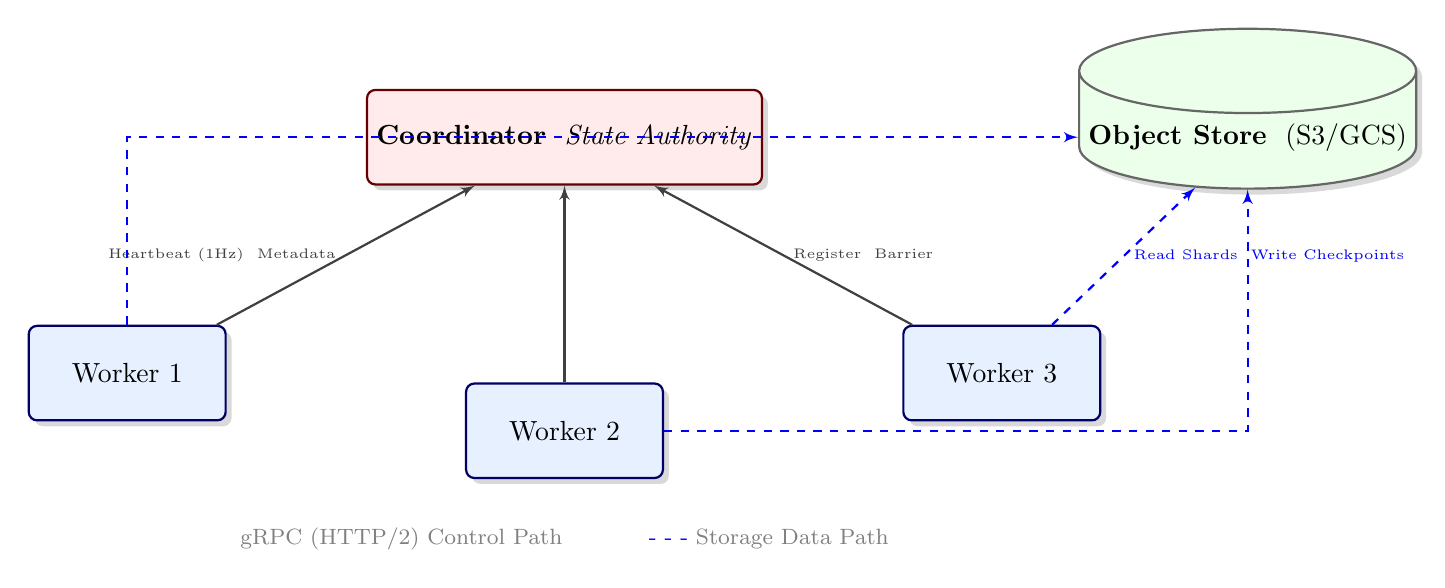
\begin{tikzpicture}[node distance=2.5cm]

    % Nodes
    \node[coordinator] (coord) {\textbf{Coordinator} \ \textit{State Authority}};
    
    \node[worker, below left=of coord] (w1) {Worker 1};
    \node[worker, below=of coord] (w2) {Worker 2};
    \node[worker, below right=of coord] (w3) {Worker 3};
    
    \node[storage, right=4cm of coord] (s3) {\textbf{Object Store} \ (S3/GCS)};

    % Connections
    \path[line] (w1) -- node[midway, left, font=\tiny, align=center] {Heartbeat (1Hz) \ Metadata} (coord);
    \path[line] (w2) -- (coord);
    \path[line] (w3) -- node[midway, right, font=\tiny, align=center] {Register \ Barrier} (coord);

    \path[dashedline, blue] (w1) |- (s3);
    \path[dashedline, blue] (w2) -| (s3);
    \path[dashedline, blue] (w3) -- node[midway, right, font=\tiny, color=blue] {Read Shards \ Write Checkpoints} (s3);

    % Legend
    \node[below=0.5cm of w2, font=\footnotesize, color=gray] {gRPC (HTTP/2) Control Path \\ \hspace{1cm} {\color{blue} - - -} Storage Data Path};

\end{tikzpicture}
\caption{Hub-and-Spoke Control Plane with Direct-to-Storage Data Plane}
\label{fig:topology}
\end{figure}

\section{Coordinator Service (Control Plane)}

The Coordinator is a high-performance, stateless-logic server that maintains the cluster state in memory. It is implemented in Rust to guarantee memory safety and predictable latency under load.

\subsection{State Management (The DashMap Pattern)}
To support thousands of concurrent heartbeats without locking contention, the Coordinator eschews global Mutexes in favor of sharded concurrent maps (\texttt{DashMap}).

\begin{lstlisting}[language=Rust]
pub struct CoordinatorState {
    // Sharded map for O(1) concurrent access
    pub workers: DashMap<WorkerId, WorkerState>,
    
    // Atomic counters for global statistics
    pub active_workers: AtomicUsize,
    
    // Barrier generation counter for synchronization
    pub current_barrier_generation: AtomicU64,
}
\end{lstlisting}

\subsection{Failure Detector Logic}
The system employs a \textit{Phi Accrual Failure Detector} style logic, simplified for deterministic thresholds. 
\begin{itemize}
    \item \textbf{Heartbeat}: Workers stream heartbeats on a gRPC bidirectional stream.
    \item \textbf{TTL}: Each heartbeat updates a `last_seen` timestamp.
    \item \textbf{Reaper}: A background Tokio task scans the `workers` map every 500ms. If `now - last_seen > 30s`, the worker is atomically evicted.
\end{itemize}

\section{Distributed Data Sharding (Data Plane)}

A critical innovation is the use of \textbf{Consistent Hashing} for dataset sharding. This allows the cluster to resize dynamically (elasticity) without requiring a full cluster restart or manual re-sharding.

\subsection{The Ring Algorithm}
We utilize a virtual-node consistent hashing ring to map $S$ data shards to $N$ workers.

\begin{equation}
    Worker(Shard_i) = \text{lookup\_ring}(\text{Hash}(DatasetID \oplus Shard_i))
\end{equation}

\textbf{Why this matters for production:}
\begin{enumerate}
    \item \textbf{Minimal Disruption}: If one worker fails, only $1/N$ of the shards (its share) are reassigned. The remaining $(N-1)/N$ shards stay with their current workers, preserving local caches.
    \item \textbf{Statelessness}: The Coordinator does not need to store a mapping table of size $S$. It only stores the active worker list. The assignment is algorithmically derived.
\end{enumerate}

\subsection{Epoch Shuffling & Determinism}
To ensure statistical convergence, data must be shuffled every epoch.
\begin{itemize}
    \item \textbf{Global Seed}: A random seed $R$ is generated per epoch.
    \item \textbf{Permutation}: The shard index is permuted: $Shard'_i = \text{Permute}(i, R)$.
    \item \textbf{Assignment}: The permuted ID is fed into the hash ring.
\end{itemize}
This guarantees that while the assignment is random per epoch, it is \textbf{deterministic} for all workers given the seed.

\section{Asynchronous Checkpointing Pipeline}

Blocking the training loop to write gigabytes of model weights to S3 is unacceptable. We implement a "Snapshot-and-Upload" mechanism.

\subsection{Zero-Copy FFI}
When Python calls `save_async(state_dict)`, the Rust extension performs the following without copying tensor data where possible (using PyTorch's shared memory pointers):

\begin{figure}[H]
\centering
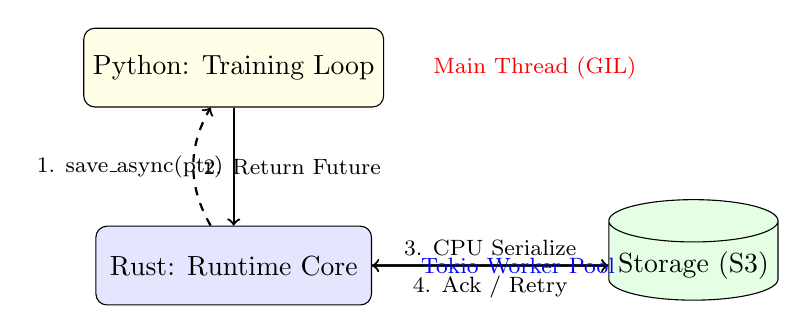
\begin{tikzpicture}[node distance=1.5cm]

    % Nodes
    \node[draw, rectangle, rounded corners, fill=yellow!10, minimum width=3.5cm, minimum height=1cm] (py) {Python: Training Loop};
    
    \node[draw, rectangle, rounded corners, fill=blue!10, minimum width=3.5cm, minimum height=1cm, below=of py] (rust) {Rust: Runtime Core};
    
    \node[draw, cylinder, shape border rotate=90, aspect=0.25, fill=green!10, right=3cm of rust] (disk) {Storage (S3)};

    % Interactions
    \draw[->, thick] (py) -- node[left, font=\footnotesize] {1. save\_async(ptr)} (rust);
    \draw[->, thick, dashed] (rust) to[bend left] node[right, font=\footnotesize] {2. Return Future} (py);
    
    \draw[->, thick] (rust) -- node[above, font=\footnotesize] {3. CPU Serialize} (disk);
    \draw[->, thick] (disk) -- node[below, font=\footnotesize] {4. Ack / Retry} (rust);

    % Annotations
    \node[right=0.5cm of py, font=\footnotesize, color=red] {Main Thread (GIL)};
    \node[right=0.5cm of rust, font=\footnotesize, color=blue] {Tokio Worker Pool};

\end{tikzpicture}
\caption{Non-Blocking Checkpoint Architecture}
\end{figure}

\begin{enumerate}
    \item \textbf{Serialize}: The state dict is serialized to an in-memory buffer (RAM).
    \item \textbf{Spawn}: A Tokio task takes ownership of the buffer.
    \item \textbf{Return}: Control returns to Python immediately (< 10ms).
    \item \textbf{Upload}: The background task streams the buffer to S3 using multipart uploads.
\end{enumerate}

\section{Reliability & Production Hardening}

This section details the architectural features specifically designed to mitigate production failures.

\subsection{Network Resilience (gRPC Interceptors)}
All inter-node communication is wrapped in a robust middleware layer:
\begin{itemize}
    \item \textbf{Exponential Backoff}: Retries with jitter (base 100ms, max 5s) for transient network partitions.
    \item \textbf{Keep-Alive}: HTTP/2 PING frames sent every 10s to prevent load balancer idle timeouts.
    \item \textbf{Compression}: GZIP compression enabled for large metadata payloads (reducing bandwidth by ~60\%).
\end{itemize}

\subsection{Zombie Process cleanup}
To prevent resource leaks in a Kubernetes environment:
\begin{itemize}
    \item The Rust runtime installs a `SIGTERM` handler.
    \item Upon termination signal, it attempts a "Graceful Departure" RPC to the coordinator.
    \item A "Dead Man's Switch" thread monitors the parent Python process. If the parent dies (segfault), the Rust runtime automatically terminates to release GPU resources.
\end{itemize}

\end{document}
